
While considering ``straight-line'' traces may have some utility in player
analytics, a more exciting prospect for formalizing game interactions as
program constructs is the possibility of
encoding {\em parameterized} sequences of actions that may carry out
complex tasks. After all, games with rich player action languages afford
modes of exploratory and creative play: consider item crafting in
Minecraft~\cite{minecraft}, puzzle solving in Zork~\cite{blank1980zork}, or
creating sustainable autonomous systems like a supply chain in
Factorio~\cite{factorio}, a farm in Stardew Valley~\cite{stardew}, or a
transit system in Mini Metro~\cite{minimetro}.  Each of these activities
asks the player to understand a complex system and construct multi-step
sequences of actions to accomplish specific tasks. From the player's
perspective, these plans are constructed from higher-level activities,
such as {\em growing a crop} or {\em constructing a new tool}, which
themselves are constructed from the lower level game intent language.

A language, as we have formalized it, gives us the atomic pieces from which
we can construct these sequences, like Lego bricks can be used to construct
reconfigurable components of a house or spaceship. {\em Compositionality}
in language design is the principle that we may understand the meaning and
behavior of compound structures (e.g. sequences) in terms of the meaning
and behavior of each of its pieces (e.g. actions), together with the
meaning of how they are combined (e.g. carried out one after the other, or
in parallel). In this section, we describe how we might make sense of {\em
player skills} in terms of programs written in a more complex version of
the player language.

\begin{figure}
  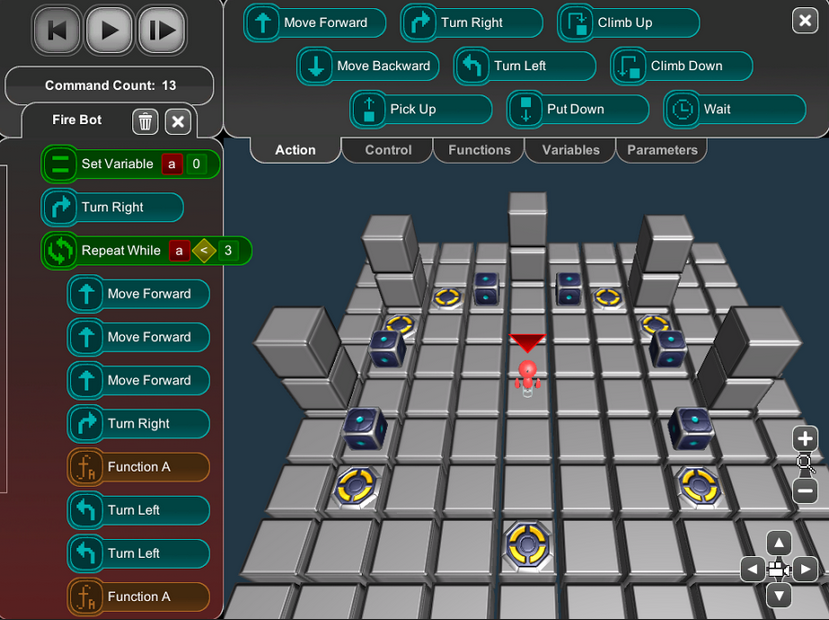
\includegraphics[width=0.45\textwidth]{bots.png}
  \caption{A screenshot from BOTS, an educational game in which players
  write programs to direct a player avatar.}
  \label{fig:bots}
\end{figure}

Such programs might be integrated into a game's mechanics so that a player
explicitly writes such programs, as in the BOTS game, an interactive
programming tutor that asks players to write small imperative programs that
direct an avatar within a virtual world~\cite{hicks2012creation} (see
Figure~\ref{fig:bots}), or Cube
Composer\footnote{\url{http://david-peter.de/cube-composer/}}, in which
players write functional programs to solve puzzles. However, for now, we
primarily intend this account of player skills as a conceptual tool.

\subsection{Example: Stardew Valley}

\begin{figure}
  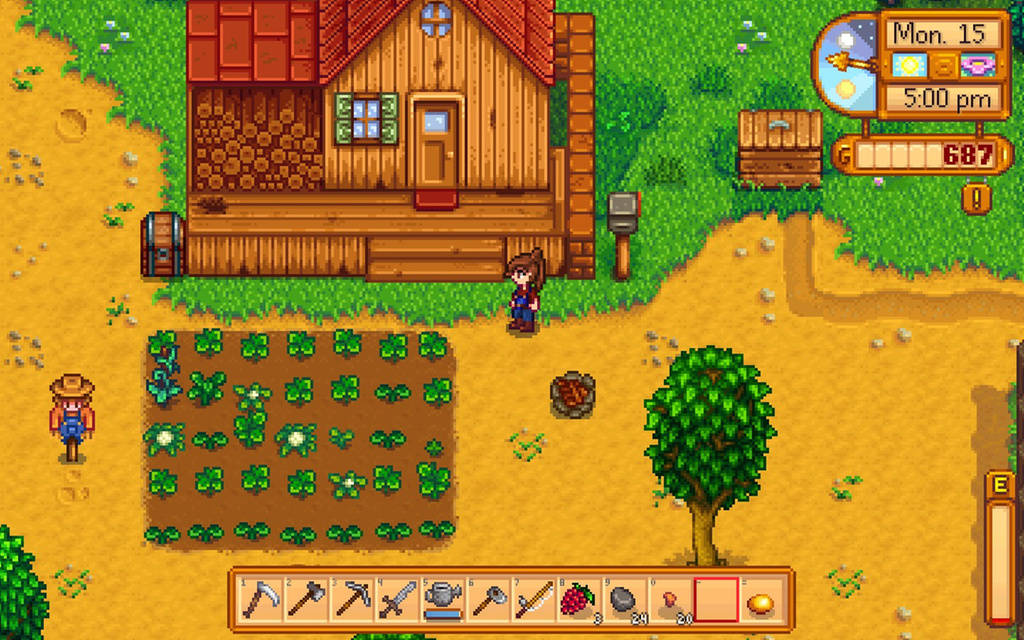
\includegraphics[width=0.45\textwidth]{stardew-valley.png}
  \caption{A screenshot from Stardew Valley showing the player's farm,
  inventory, and avatar.}
  \label{fig:stardew}
\end{figure}

Our initial $\{\cmove, \ctake\}$ example is too simple to craft really
compelling examples of complex programs, so here we examine
Stardew Valley and its game language for the sake of considering player
skills. In Stardew Valley, the player has an inventory that permits varied
interactions with the world, beginning a number of tools for farming (axe,
hoe, scythe, pickaxe) which do different things in contact with the
resources in the surrounding environment; most include extracting some
resource (wood, stone, fiber, and so on), which themselves enter the
player's inventory and can be used in further interaction with the game
world. The player's avatar is shown on-screen, moved by WASD.  There are
also context-sensitive interactions between the player and non-player
characters (NPCs), interfaces through which new items may be purchased
(shops), and mini-games including fishing (fish may also be sold at high
value). See Figure~\ref{fig:stardew} for a typical player view of the game.

While a full account of the language that this game affords the player is
beyond the scope of this paper, we include a representative sample of the
actions and affordances found in this game that may be used to construct
player skills.
These include: directional avatar movement within and between
world ``rooms,'' point-and-click actions for selecting items in
one's inventory, and interacting with in-room entities. 

The player avatar must be near an entity for the player to interact with
it. They can then either $\syn{apply}$ the currently-selected inventory
item to the in-world entity with a left-button click, or right-button
click, which does something based on the entity type, e.g. doors and chests
open, characters speak, and collectible items transfer to the player's
inventory. We refer to this last action as $\syn{inquire}$. We also note
that, for the sake of our example, movement towards an entity and movement
offscreen (towards another room) are the only meaningful and distinct types
of movement, which we refer to as $\syn{move\_near}$ and
$\syn{move\_offscreen}$. These actions yield the following syntax:

% (an item is something held, an entity is something in the world)
\begin{eqnarray*}
intent &::=& \syn{select} \param{item}\\
       &\mid& \syn{apply} \param{entity}\\
       &\mid& \syn{inquire} \param{entity}\\
       &\mid& \syn{move\_near} \param{entity}\\
       &\mid& \syn{move\_offscreen} \param{direction}
\end{eqnarray*}

We leave the definition of items and entities abstract, but we could
imagine it to simply list all possible items and entities in the world as
terminal symbols.  
%
From these atomic inputs, we can start to construct higher-level actions
performed in the game most frequently---tilling land, planting seeds,
conversing with NPCs, and so on. These blocks of code may be assigned names
like functions to be called in many contexts:

% we want to accurately reflect the
% {\em extensibility} of Stardew Valley's player language by describing the
% general system from which these actions are derived. In other words, rather
% than having each instance of such an action be a special case that a player
% must learn how to speak as an independent vocabulary term, instead, they
% learn it through {\em composing} the pre-existing constructs of selecting items
% and applying them to objects in the world. For example: (XXX explain this
% more)
% 
% XXX semantics?

% Higher-level actions:
\begin{verbatim}
action till = 
  select hoe; move_near hard_ground; 
  apply hard_ground
action plant = 
  select seeds; move_near tilled_ground; 
  apply tilled_ground
action mine = 
  select pickaxe; move_near rock; apply rock
action enter_shop = 
  move_near shop; inquire door(shop)
action talk = move_near npc; inquire npc
\end{verbatim}

In turn, these larger skill molecules may be combined to accomplish
specific tasks or complete quests.

\subsection{Branching programs as skills and strategies}

Note that we have naively sequenced actions without consideration for the
game's response. This approach to describing player skills does not take
into account the possbility of a failed attempt, such as attempting to mine
when there are no rocks on the current screen. One could simply assign a
semantics to these sequences of action that threads failure through the
program---if we fail on any action, the whole compound action fails.

However, we can go further with describing robust player skills and
strategies if we consider the possibility of {\em handling} failure, a
common feature of day-to-day programming and indeed of gameplay. Recall our
simplified game response language consisting of two possibilities,
$\syn{success}$ and $\syn{failure}$. We can introduce a $\syn{case}$
construct into our language to handle each of these possibilities as a
distinct branch of the program:

\begin{verbatim}
action mine = 
  response = select pickaxe;
  case(response):
    success => {
      response' = move_near rock;
      case(response'):
          success => apply rock;
        | failure => fail;
    }
  | failure => fail;
\end{verbatim}

However, to avoid handling failure at every possible action, a better
approach is to explicitly indicate as parameters the world resources that
each action needs in order to complete successfully.
The overall action definition for mining, or example, would
require as a precondition to the action that a pickaxe is
available in the player inventory and a rock is in the ssme room. The
actions for selecting the pickaxe and moving near the rock would depend on
these resources, and the game response language could include the resources
it guarantees as outputs. Then we can write the program using simpler
notation that refers to resource dependencies of the appropriate type
(using notation \verb|resource : type|):

\begin{verbatim}
action mine(p:pickaxe, r:rock) = 
  select p; move_near r; apply r
: mineral
\end{verbatim}

% The task of defining a language of compound actions enters novel territory
% in programming language design, because compound player actions
% are typically interleaved with game response: the player does not have full
% knowledge of how the game world works, so she experiments with its
% affordances, develops a model for which actions map to which responses, and
% then plans accordingly. 
% Players therefore often create ad-hoc plans on the basis of
% real-time game responses, gradually learning to form complex plans by
% thinking further in advance about their consequences.

This notation together with a branching \verb|case| construct
scales to include nondeterminism in the game world, such as the fishing
minigame in Stardew Valley: the game always eventually tells the player
that something is tugging at her line, but some portion of the time it is a
fish while the rest of the time it is trash.  These constructs can also
account for incomplete player mental models, such as knowing that one must
water her seeds repeatedly day after day in order to grow a crop, but not
knowing how many times.

Below, we present a notation that accounts for these aspects of player
skills: a \verb|do ... recv ...| notation indicates a command and then
binds the response to a {\em pattern}, or structured set of variables,
which can then be case-analyzed.
Our first example is watering a crop until it may be harvested:

\begin{figure}
  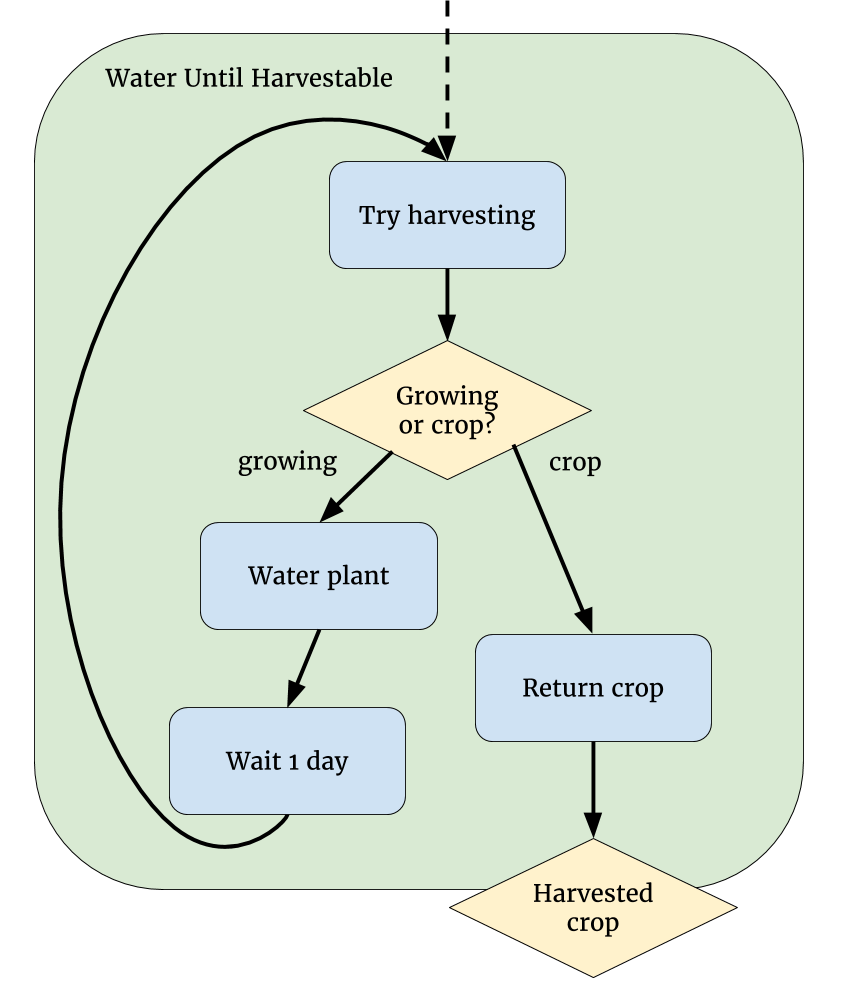
\includegraphics[width=0.4\textwidth]{sdv-water-harvest.png}
  \caption{Watering a crop until it may be harvested.}
  \label{fig:harvest}
\end{figure}

\begin{verbatim}
action water_until_harvestable[t](p: planted(t))
: crop(t) =
  do try_harvest(p)
    recv <result: crop(t) + growing(t)>.
      case result of
        c:crop(t) => c
      | g:growing(t) => 
          water(g, w); 
          wait(day); 
          try_harvest(g)
\end{verbatim}
See Figure~\ref{fig:harvest} for a control flow diagram of this code.

The next example shows a parallel construct \verb/||/, which can be used to
compose actions with distinct dependencies, as well as
how an action definition may use other action definitions by threading
resource dependencies through as arguments:

\begin{figure}
  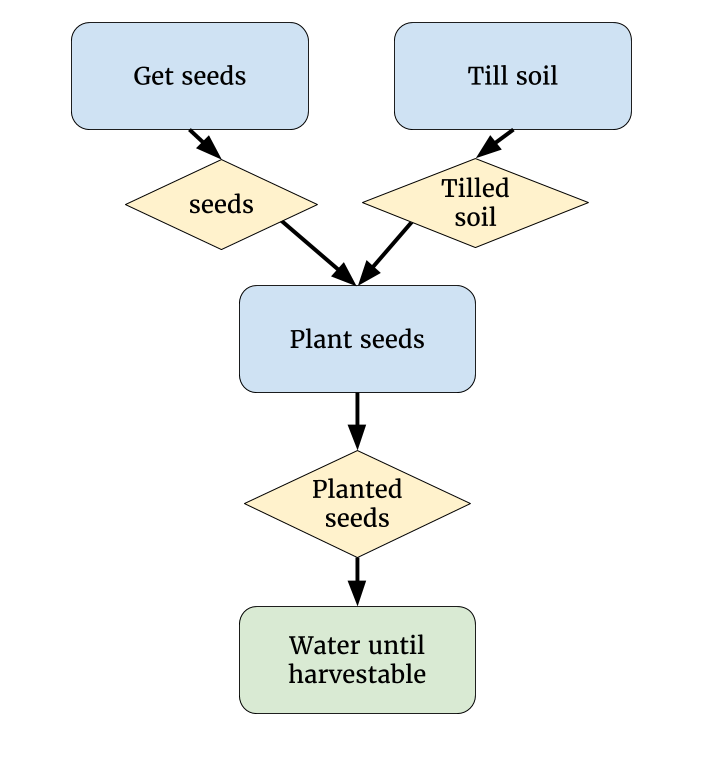
\includegraphics[width=0.4\textwidth]{sdv-grow-crop.png}
  \caption{Growing a crop.}
  \label{fig:grow}
\end{figure}

\begin{verbatim}
fun grow_crop[t : croptype](s:soil, w:watering_can)
: crop(t) =
  do
    get_seeds(t) || till_soil(s)
  recv <s: seeds(t), g: tilled_soil>.
    do
      plant(s, g)
    recv <p: planted(t)>.water_until_harvestable(p)
\end{verbatim}
See Figure~\ref{fig:grow} for a control flow diagram of this code.

 
% This is one of the ways games are said to teach us {\em systems thinking}:
% by showing us, piece by piece, what each part of a system accomplishes in
% isolation, then framing one's activity within an over-arching goal, the
% player must reason about her actions' effects on the world and how they
% interact with one another, not just how they behave in isolation. We
% observe the cause-and-effect behavior and start to form {\em higher-level
% plans} in terms of the skills we learn how to do: instead of {\em plant
% crop; water crop; harvest crop; sell crop} we may refer to the collective
% action as {\em farming} and incorporate this action with other high-level
% skills (mining, fishing) into a plan for how our character should spend her
% day.
% 
% One possible plan she can take is to scavenge the local wildlife: after
% using the scythe on enough wild brush, she may find wild seeds for free,
% which may be planted. Another option is to purchase some inexpensive seeds
% at the general store. Then she must learn to grow the crop: tilling earth,
% optionally fertilizing it, placing seeds in the ground, and then watering
% it day after day (in between which other tasks may be accomplished).
% Finally she must harvest the crop and take it to market to sell, then
% repeat the process with a stronger financial foundation.
% 
% XXX continue

% \subsection{Stardew Valley Bots}

% \begin{figure*}
%   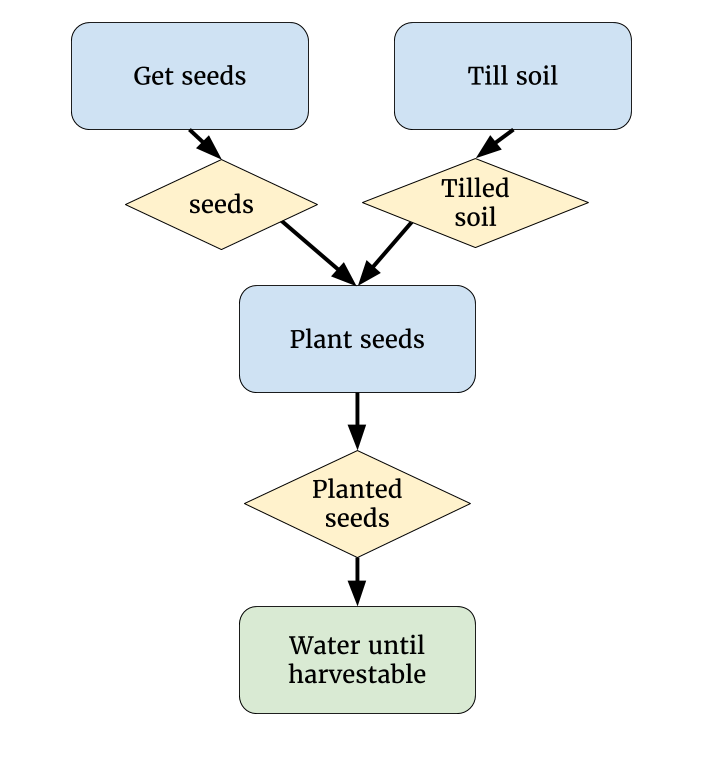
\includegraphics[width=0.4\textwidth]{sdv-grow-crop.png}
%   \quad
%   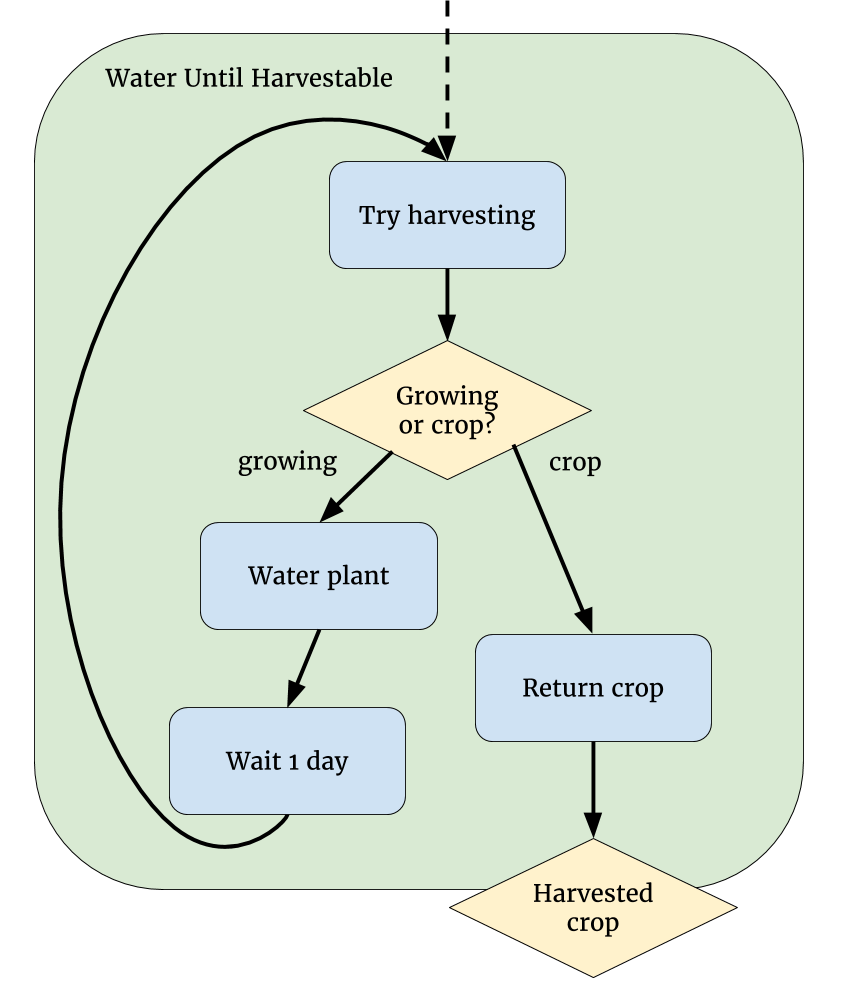
\includegraphics[width=0.4\textwidth]{sdv-water-harvest.png}
%   \caption{Control flow diagrams describing how Stardew Valley skills can
%     be described and composed. Yellow diamond-shaped nodes indicate game
%     responses and resources from the game environment, while blue
%     round-rect nodes are player actions. Green round-rect shapes indicate
%     compound action definitions and invocations.}
% 
% \end{figure*}



% Fishing:
% \begin{verbatim}
% fun get_fish(r:rod, w:water, nf:notfishing) 
% : rod * water * notfishing * fish
% =
%   do  
%     go_fish(r,w,nf)
%   recv <r:rod, w:water, ft : (fish*notfishing)+(trash*notfishing)>.
%     case ft of
%       inl <f, nf> => <r, w, nf, f>
%     | inr <t, nf> => do dispose t recv (). get_fish(r,w,nf)
% \end{verbatim}
% 

